\section{Design}
The \dns cache manipulation method is largely derived from the method used in "The Internet Connected Project", the project preceding this one \cite{Fakult2019}. The method makes use of two sets of geographically diverse \dns servers: one list each of recursive and authoritative servers. The basic principle rests on the concept of making requests directly to each of the recursive servers that \textit{must} make their way to the authoritative ones and deducing the time between the two. As \dns includes no mechanism for reporting the time taken between two servers, \dns cache manipulation must rely on the \rtt from when the local request is dispatched to when an answer is received.

\subsection{Collection Stages}\label{sec:dns_design_collection_stages}

Collecting data via \dns cache manipulation takes six stages of processing: three for pre-processing and three to make the actual measurements. The preparatory stages, server confirmation, reliability checks, and geolocation, eliminate servers that are not appropriate to include in the study.

\begin{figure}[h]
    \centering
    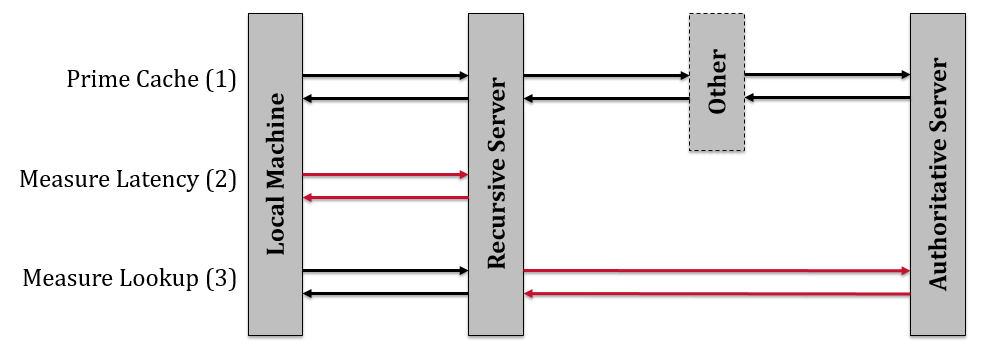
\includegraphics[width=\textwidth]{dns/diagrams/dns_cache_manipulation_diagram.png}
    \caption{DNS cache manipulation stages}
    \label{fig:dns_cache_manipulation_stage_diagram}
\end{figure}

\autoref{fig:dns_cache_manipulation_stage_diagram} shows the three stages required for data collection: priming the \dns cache, measuring latency to the recursive \dns server, and measuring the lookup time. We will now discuss all five stages in more detail.

\subsubsection{Confirmation of Server Status and Type}\label{sec:dns_des_server_conf}
Prior to running any tests, two lists of candidate recursive and authoritative servers are fed into tools that confirm their status as usable servers. For recursive servers, this process confirms that they are indeed public recursive servers. For authoritative candidates, it verifies that the server provides an answer for the domain it is expected to.

\subsubsection{Testing Reliability}
\todo{A diagram or two would definitely help. Also CoV def.}
Before actually using any of the servers for testing, we tested their reliability -- i.e. how consistent their response times were under constant parameters. After making repeated requests to each server, that in theory should have similar response times, we filter servers based on the \cv for the measured response times. This eliminated any servers with high variation from the testing. For recursive servers, priming the cache (see below) and then making repeated requests for the primed value served as the repeated requests. For authoritative servers, this was accomplished by making repeated requests for a random subdomain that the servers are authorities for through the \wpi recursive \dns server. This server is close enough to the machine we ran the tests on that the lag was minimal. The justification for running the filtering prior to testing is that each server included in the test increased the time required to run the entire test suite exponentially, as each recursive server was paired with each authoritative server.

\subsubsection{IP Geolocation}
Just as in the other methods described in this report, \dns cache manipulation utilized IP geolocation provided by MaxMind to determine the location of the servers under test.

\subsubsection{Priming the DNS Cache} 
The first step of the actual testing involves priming the target recursive server's cache. Say the target recursive server's \ip address is \texttt{1.2.3.4} and the target authoritative server provides answers for \texttt{example.com}. By making a \dns query to \texttt{1.2.3.4} for \texttt{example.com}, we get the target \dns server to cache the answer to the query.

\subsubsection{Measuring Latency} 
After the target recursive server has cached the answer for the query for \texttt{example.com}, it will use that cached answer to respond to subsequent requests without making any iterative requests. We can then make another request, identical to the one in the priming stage, and time it. To get a latency measurement, we do this several times back to back and take the lowest value, which indicates the best possible latency between the machine the measurements are being taken on and the recursive server.

\subsubsection{Measuring the Total RTT} 
The final step in the process is to measure the \rtt between the local machine and the target authoritative server and subtract the latency to get the final result. To do this, we make a query to the recursive server for \texttt{random.example.com}, where \texttt{random} is a randomly generated sub-domain that is unlikely to actually exist on the targeted domain. This random sub-domain forces the recursive server to get an answer. Because it already knows the authoritative server for \texttt{example.com}, it can skip the process of querying the root and \texttt{.com} servers and make an immediate query to the server for \texttt{example.com}. We measure the time for this entire process and then subtract the previously measured latency, leaving only the time between the target recursive server and the target authoritative server, which is recorded.